\clearpage
\section{Background}\label{sec-background}

Build systems automate the execution of simple repeatable tasks for individual
users, as well as for large organisations. There are software build systems,
such as \Make~\cite{feldman1979make}, \Shake~\cite{mitchell2012shake} and
\Bazel~\cite{bazel}, as well as various incremental calculation engines, such
as \Excel~\cite{advanced_excel}. In this section we use these four examples to
introduce main domain-specific notions and requirements. Other notable examples
of build systems and their relation to these four will be discussed
in~\S\ref{sec-related} and~\S\ref{sec-conclusions}.

\subsection{The venerable \Make: static dependencies and file modification times}
\label{sec-background-make}

\Make\footnote{There are numerous implementations of \Make and none comes with a
formal specification. In this paper we therefore use a simple and sensible
approximation to a real \Make that you might find on your machine.} was developed
more than 40 years ago to automatically build software libraries and executable
programs from source code. It uses \emph{makefiles} to describe tasks (often
referred to as \emph{build rules}) and their dependencies in a simple text form.
For example:

\vspace{1mm}
\begin{minted}[xleftmargin=10pt]{makefile}
util.o: util.h util.c
    gcc -c util.c

main.o: util.h main.c
    gcc -c main.c

main.exe: util.o main.o
    gcc util.o main.o -o main.exe
\end{minted}
\vspace{1mm}

\noindent
The above makefile lists three tasks: (i) compile a utility library comprising
files \cmd{util.h} and \cmd{util.c} into \cmd{util.o} by
executing\footnote{In this example we treat \cmd{gcc} as a pure function for the
sake of simplicity. In reality, there are multiple versions of \cmd{gcc} and the
actual binary that is used to compile and link files is often also listed as a task
dependency.} the command \cmd{gcc -c util.c}, (ii) compile the main source file
\cmd{main.c} into \cmd{main.o}, and (iii) link object files \cmd{util.o} and
\cmd{main.o} into the executable \cmd{main.exe}. The makefile contains the
complete information about the \emph{task dependency graph}, which is shown in
Fig.~\ref{fig-make}(a).

\begin{figure}[h]
\begin{subfigure}[b]{0.32\linewidth}
\centerline{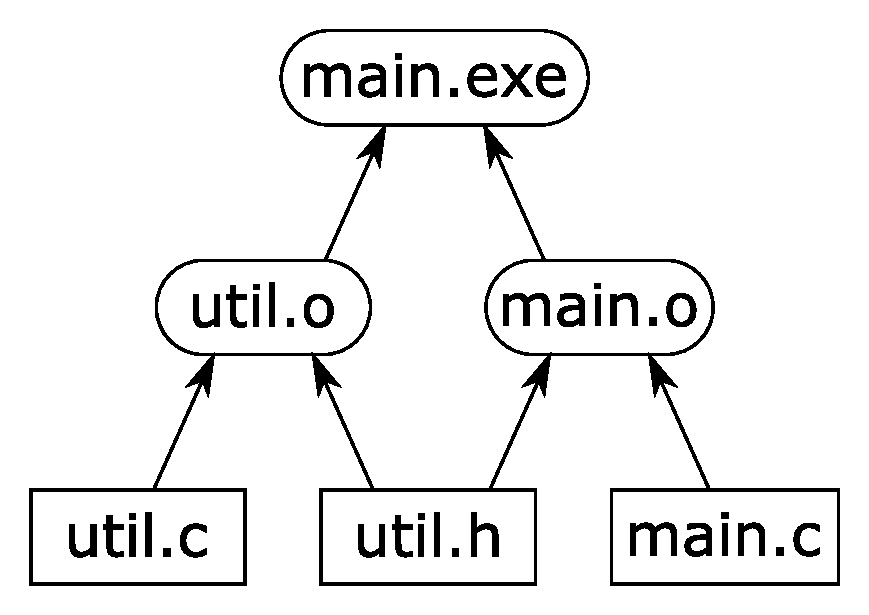
\includegraphics[scale=0.28]{fig/make-example.pdf}}
\caption{Task dependency graph}
\end{subfigure}
\begin{subfigure}[b]{0.32\linewidth}
\centerline{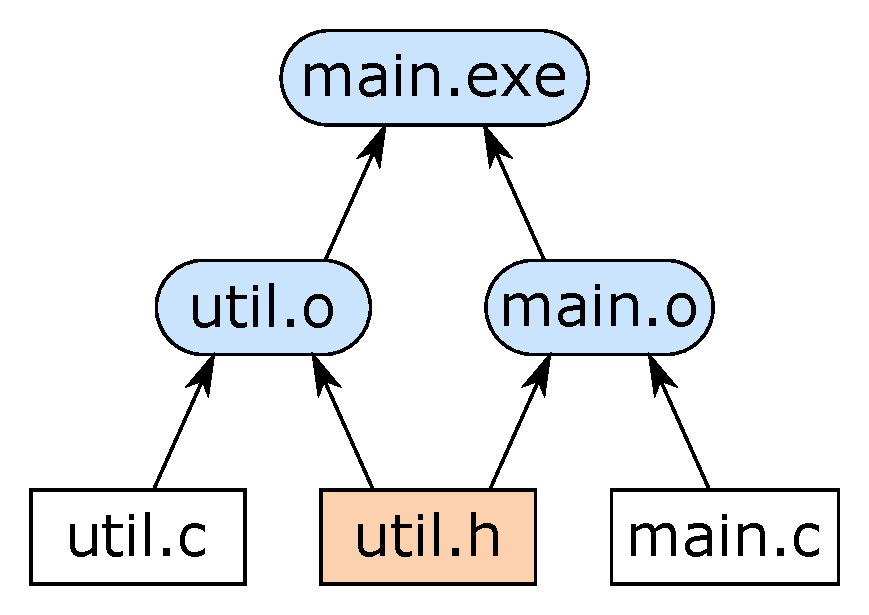
\includegraphics[scale=0.28]{fig/make-example-full.pdf}}
\caption{Full rebuild}
\end{subfigure}
\begin{subfigure}[b]{0.32\linewidth}
\centerline{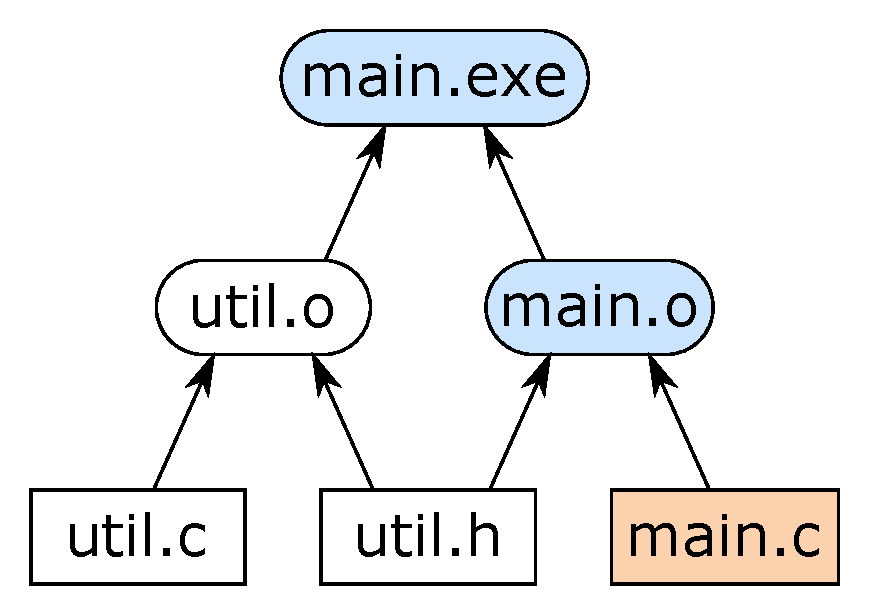
\includegraphics[scale=0.28]{fig/make-example-partial.pdf}}
\caption{Partial rebuild}
\end{subfigure}
\caption{A task dependency graph and two build scenarios. Input files are shown as
rectangles, intermediate and output files are shown as rounded rectangles. Dirty
inputs and files that are rebuilt are highlighted.
\label{fig-make}}
\end{figure}

If the user modifies the sources of the utility library and runs \Make, it will
perform a full rebuild, because all three tasks transitively depend on the
library, as illustrated in Fig.~\ref{fig-make}(b). On the other hand, if the
user modifies \cmd{main.c} then a partial rebuild is sufficient: indeed, the
file \cmd{util.o} does not need to be rebuilt, since its inputs have not
changed, see Fig.~\ref{fig-make}(c). Files that have changed since the previous
build are called \emph{dirty}.

The requirement to \emph{execute tasks at most once and only if they transitively
depend on dirty inputs} is essential for build systems, it is their raison
d'\^etre. We will call build systems that satisfy this requirement \emph{minimal}.

To achieve minimality \Make relies on two main ideas. First, it uses \emph{file
modification time} to detect the files that are dirty: a file is marked dirty if
it was modified since the previous build. Second, it constructs a complete task
dependency graph from the information contained in the makefile and executes
tasks in a \emph{topological order}.

Note that it is not always possible to know the dependencies of a task upfront,
or \emph{statically}. To demonstrate this, let us add another task to the above
makefile:

\vspace{1mm}
\begin{minted}[xleftmargin=10pt]{makefile}
release.tar: main.exe README
    tar -cf release.tar main.exe README
\end{minted}
\vspace{1mm}

\noindent
So far so good: if either \cmd{main.exe} or \cmd{README} is dirty, \Make will
recreate the release archive. But now imagine that we need to specify the files
that go into \cmd{release.tar} in a text file \cmd{release.txt}. The dependencies
of \cmd{release.tar} are no longer known statically: they \emph{depend on the
content} of \cmd{release.txt}, which might not even exist before the build
starts, e.g. if it is produced by concatenating input files \cmd{release-bins.txt}
and \cmd{release-docs.txt}. Alas, makefiles cannot express such \emph{dynamic
dependencies}, requiring ad hoc workarounds such as \emph{build phases}, which
are problematic~\cite{hadrian}.

\subsection{\Excel: dynamic dependencies at the cost of minimality}
\label{sec-background-excel}

\Excel is a build system that can deal with dynamic dependencies albeit at the
cost of sacrificing minimality. Consider the following spreadsheet comprising
four input cells \cmd{A1-A3} and \cmd{B1}, and a single task computing the sum
of values \cmd{A1} $+\cdots+$ \cmd{An}, where \cmd{n} is specified indirectly in
\cmd{B1}:

\vspace{1mm}
\begin{minted}[xleftmargin=10pt]{bash}
A1 = 10
A2 = 20
A3 = 30
B1 = 2
C1 = SUM(A1:INDIRECT("A" & B1))
\end{minted}
\vspace{1mm}

\noindent
The output \cmd{C1} here is analogous to the \cmd{release.tar} from the previous
example: one cannot statically determine the dependencies of the associated task.
To deal with this, \Excel takes a simple conservative approach: it marks all
cells with dynamic dependencies as dirty and therefore always recomputes them
during a rebuild. This guarantees that the build result is correct, but clearly
violates the minimality requirement: if the user modifies \cmd{A3}, \Excel will
recompute \cmd{C1} even though it does not transitively depend on \cmd{A3}.

Note that \Excel's approach to marking cells as dirty is a relatively minor
variation of the approach used by \Make: a cell is considered dirty if it was
modified since the previous build \emph{or if it is volatile}, where the notion
of volatility includes dynamic dependencies, as well as \emph{non-determinism}
that will be discussed in~\S\ref{sec-non-determinism}. We therefore put both
\Make and \Excel in the same category of build systems that associate a
\emph{dirty bit} with every file or cell. (To avoid the ``file or cell''
nuisance, we introduce the abstract notion of \emph{keys}
in~\S\ref{sec-background-vocabulary}.)

\Excel's recalculation algorithm~\cite{excel_recalc} on the other hand is
significantly different from \Make. Since it is impossible to construct the full
dependency graph upfront in the presence of dynamic dependencies, \Excel
maintains the \emph{calculation chain}, which is an approximation to the correct
topological order produced by the previous build. During recalculation, \Excel
processes cells in this order, but can \emph{defer recalculation of a cell} by
moving it down the chain when one of its newly discovered dynamic dependencies
is dirty. We discuss this algorithm in more detail in~\S\ref{sec-implementations}.

Another distinguishing feature of \Excel is \emph{self-tracking}. Most build
systems track changes of inputs and intermediate results, executing dependent
tasks whenever they change, but \Excel can also track changes in the tasks
themselves: if a formula is modified, \Excel will recompute it and propagate
the changes. Self-tracking is uncommon in software build systems, where one
often needs to manually initiate a full rebuild even if just a single task has
changed. We further discuss self-tracking in~\S\ref{sec-tracking-aspects}.

\subsection{\Shake: dynamic dependencies with no remorse}
\label{sec-background-shake}

\Shake was developed specifically to address the issue of dynamic
dependencies~\cite{mitchell2012shake} and it excels at handling them without
sacrificing the minimality requirement. Here is how one can express the task
for producing \cmd{release.tar} from the example discussed
in~\S\ref{sec-background-make}.

\vspace{1mm}
\begin{minted}[xleftmargin=10pt]{haskell}
"release.tar" %> \_ -> do
    need ["release.txt"]
    files <- lines <$> readFile "release.txt"
    need files
    system "tar" $ ["-cf", "result.tar"] ++ files
\end{minted}
\vspace{1mm}

\noindent
We first declare the static dependency on \cmd{release.txt}, then read its
content (a list of files) and depend on it, dynamically. Finally, we specify the
command to produce the resulting archive. Crucially, the archive will only be
rebuilt if one of the dependencies (static or dynamic) has changed.

\begin{figure}[h]
\begin{subfigure}[b]{0.90\linewidth}
\centerline{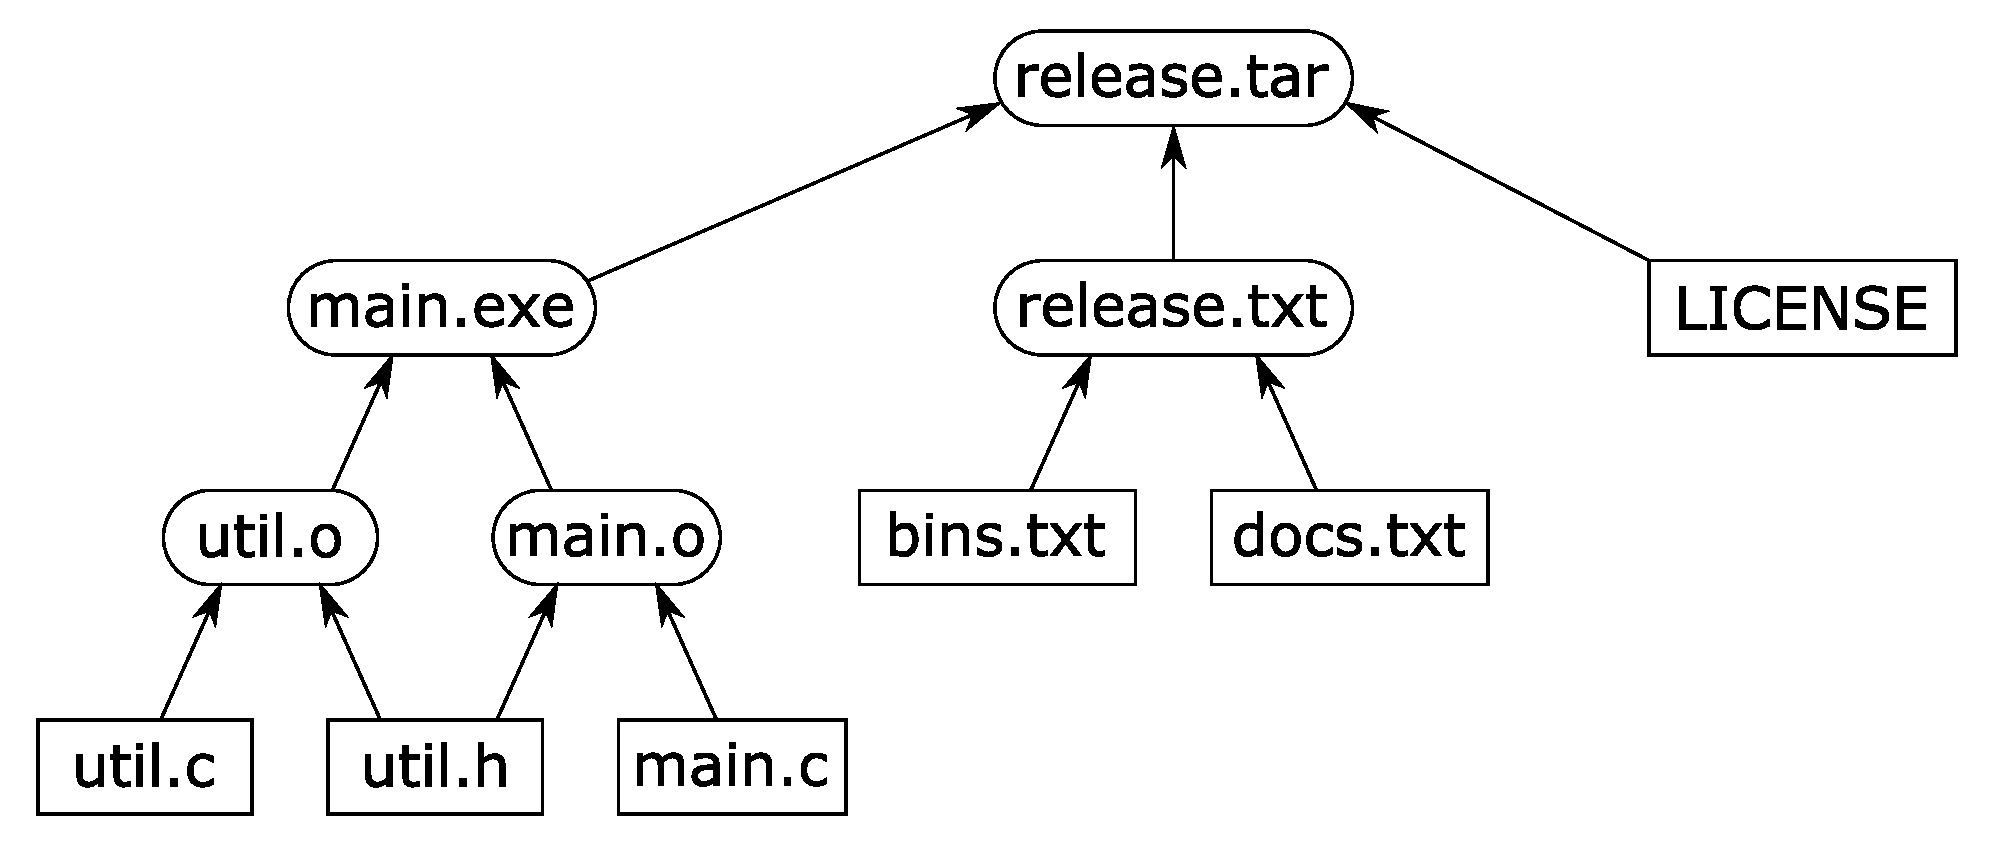
\includegraphics[scale=0.28]{fig/shake-example.pdf}}
\vspace{-1mm}
\caption{Task dependency graph produced after the previous build.}
\vspace{3mm}
\end{subfigure}
\begin{subfigure}[b]{0.90\linewidth}
\centerline{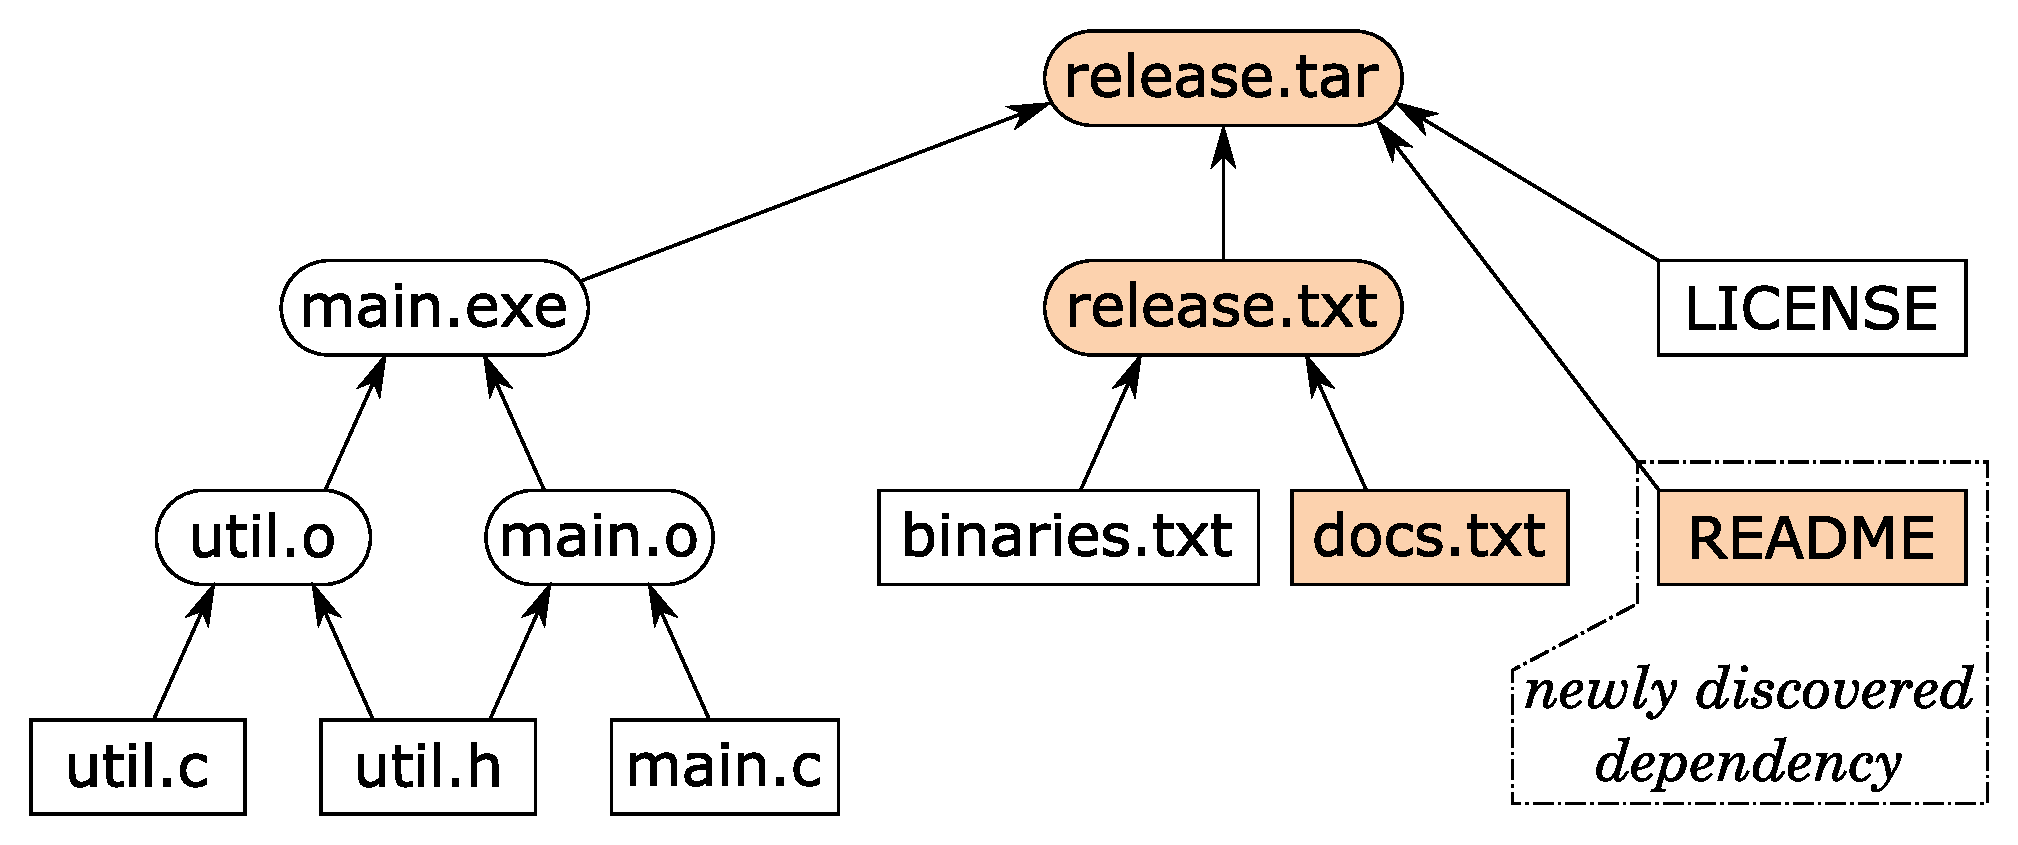
\includegraphics[scale=0.28]{fig/shake-example-rebuild.pdf}}
\vspace{-1mm}
\caption{Since \cmd{docs.txt} is dirty, we rebuild \cmd{release.txt} and
\cmd{release.tar}, discovering a new dependency.}
\end{subfigure}
\caption{Dynamic dependencies example: create \cmd{README} and add it to the
list of release documents \cmd{docs.txt}.\label{fig-shake}}
\end{figure}

\Shake's implementation is different from both \Make and \Excel in two aspects.
First, it uses the dependency graph produced in the previous build to detect
which files are dirty -- a powerful idea with a long history of use in
\emph{incremental}~\cite{demers1981incremental},
\emph{adaptive}~\cite{acar2002adaptive}, and
\emph{self-adjusting}~\cite{acar2007selfadjusting} \emph{computations} (see a
discussion in related work~\S\ref{sec-related}). Second, instead of abandoning
and deferring the computation of tasks whose rediscovered dependencies are dirty
(as \Excel does), \Shake \emph{pauses} their computation until the dependencies
are brought up-to-date. We refer to this build algorithm as \emph{recursive}.

\begin{figure}[h]
\centerline{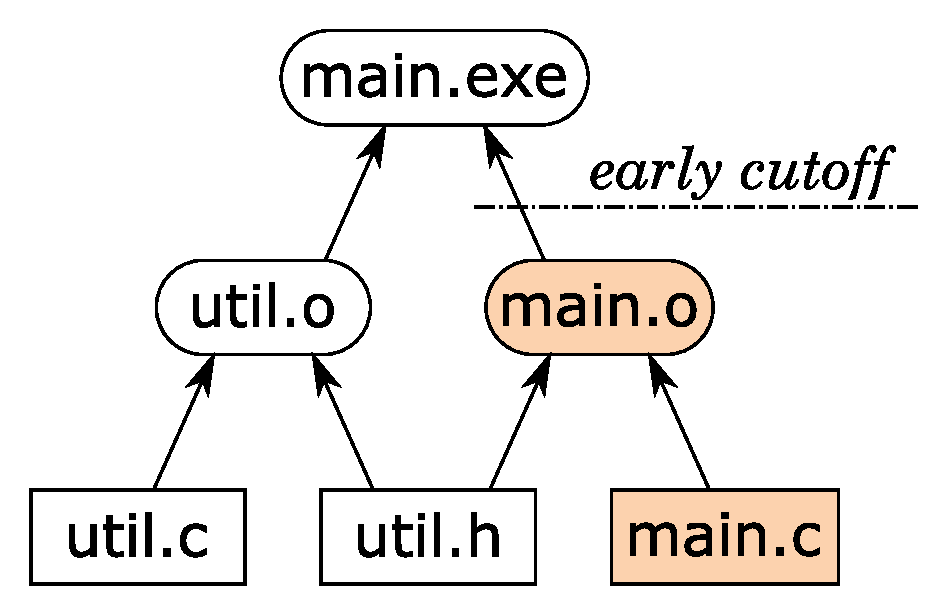
\includegraphics[scale=0.28]{fig/make-example-cutoff.pdf}}
\vspace{-2mm}
\caption{An early cutoff example: modify the source \cmd{main.c} by adding a
comment. The rebuild is stopped after detecting that \cmd{main.o} is unchanged,
which indicates that \cmd{main.exe} does not need to be rebuilt.\label{fig-cutoff}}
\end{figure}

\Shake also supports the following \emph{early cutoff optimisation}. When it
executes a task and the result is unchanged from the previous build, it is
unnecessary to execute the dependent tasks, and hence \Shake can stop a build
earlier, as illustrated in Fig.~\ref{fig-cutoff}. Not all build systems support
early cutoff: \Make and \Excel do not, whereas \Shake and \Bazel (introduced
below) do.

\subsection{\Bazel: a cloud build system}
\label{sec-background-bazel}

When build systems are used by large teams, different team members
often end up executing exactly the same tasks on their local machines.
A \emph{cloud build system} can speed up builds dramatically by
transparently sharing build results among team members. Furthermore, cloud
build systems allow one to perform \emph{shallow builds} that materialise
only end build products on a local machine, leaving all intermediates in the
cloud. This is a significant optimisation compared to \emph{deep builds}
that require all transitive dependencies of an end build product to be
locally available. % Non-cloud build systems cannot support shallow builds.

\Bazel is one of the first examples of openly available cloud build systems.
Like \Make, it does not support dynamic dependencies and can therefore benefit
from the simplicity of building tasks in the statically known topological order.
It is minimal and supports the early cutoff optimisation.

To support cloud builds, \Bazel maintains a conventional \emph{content-addressable
cache}, which can be used to fetch a previously built file given the hash of its
content, as well as \emph{dependency graphs from all previous builds}, annotated
with observed file hashes\footnote{Here we ignore the issue of limited cloud
storage resources for the sake of simplicity; in practice, old entries are
regularly evicted from the storage, as further discussed
in~\S\ref{sec-cloud-aspects}.}. The latter allows to bypass the execution of
a task, by predicting the hash of its result from the hashes of the dependencies,
and subsequently fetch the result from the cache. A concrete implementation is
provided in~\S\ref{sec-implementations}.

\subsection{Summary}
\label{sec-background-summary}

We summarise differences between four discussed build systems in
Table~\ref{tab-summary}. The `Metadata' column refers to the \emph{auxiliary
build information} persistently stored between builds by all build systems:
\begin{itemize}
    \item \Make stores file modification times, or rather, it relies on the file
    system to do that. In principle a single dirty bit is sufficient, as will be
    demonstrated in~\S\ref{sec-implementations}.
    \item \Excel stores the dirty bit as well as the calculation chain.
    \item \Shake stores the dependency graph discovered in the previous build,
    annotated with file content hashes for efficient checking of file changes.
    \item \Bazel stores all dependency graphs discovered in previous builds
    annotated with file hashes, and the content-addressable cache.
\end{itemize}

In this paper we show which build system properties are consequences of specific
implementation choices (metadata and algorithm), and how one can obtain new
build systems with desired properties by recombining parts of existing
implementations. As a compelling example, we demonstrate how to combine
advantages of \Shake and \Bazel in a cloud build system with dynamic dependencies.

\begin{table}[h]
\smaller
\centering
\begin{tabular}{l||l|c|c|c||l|l}
\hline
$\!\!$Build system & Dependencies & Minimal & Cutoff & Cloud & Metadata                       & Algorithm   $\!\!$\\\hline
$\!\!$\Make        & Static       & Yes     & No     & No    & File modification times        & Topological $\!\!$\\
$\!\!$\Excel       & Dynamic      & No      & No     & No    & Dirty cells, calculation chain & Chain, defer$\!\!$\\
$\!\!$\Shake       & Dynamic      & Yes     & Yes    & No    & Last dependency graph          & Recursive   $\!\!$\\
$\!\!$\Bazel       & Static       & Yes     & Yes    & Yes   & All dependency graphs, cache   & Topological $\!\!$\\\hline
\hline
\end{tabular}
\vspace{2mm}
\caption{Summary of build system differences.\label{tab-summary}}
\vspace{-7mm}
\end{table}

\subsection{Common vocabulary for build systems}
\label{sec-background-vocabulary}

In this section we introduce a common vocabulary for build systems that allows
us to abstract away from specific application domains, such as software
development or spreadsheets. We will use this vocabulary throughout the rest of
the paper.

\emph{Keys} are used to distinguish \emph{values}. In software build systems
keys are typically filenames, e.g. \cmd{main.c}, whereas values are file
contents (a C program source code in this case). In spreadsheets keys are cell
names, e.g. \cmd{A1}, and values are numbers, text, etc. that are typically
displayed inside cells. In Haskell code, we will use type variables \hs{k}
and \hs{v} to denote keys and values, respectively.

We use a cryptographic \emph{hash function} \hs{hash :: v -> Hash} for efficient
tracking and sharing of build results, where \hs{Hash} is an abstract data type
equipped with the equality test.

A \emph{store} associates keys to values. It is convenient to assume that a store
is total, i.e. it contains a value for every possible key. We therefore also
assume that the type of values is capable of encoding values corresponding to
non-existent keys (missing files or empty cells). This, in particular, suggests
that it is possible to \emph{depend on the absence of a value} which is a useful
feature for build systems. In addition to usual \hs{get} and \hs{put} operations,
some stores support the \hs{getHash} operation implemented more efficiently than
by hashing the result of \hs{get}. For example, GVFS (Git Virtual File
System)~\cite{gvfs} stores file hashes and downloads file contents only on demand.

Some values must be provided by the user as \emph{input}. For example,
\cmd{main.c} can be edited by the user who relies on the build system to
compile it into \cmd{main.o} and subsequently \cmd{main.exe}. End build products,
such as \cmd{main.exe}, are \emph{output} values. All other values (in this case
\cmd{main.o}) are \emph{intermediate}; they are not interesting for the user
but are produced in the process of turning inputs into outputs.
